Optimization of the nuclear fuel cycle aids in developing
a fuel cycle based on a specific objective or  multiple objectives. 
Optimization has previously been applied to the nuclear fuel 
cycle \cite{passerini_sensitivity_2012,andrianov_optimization_2019}
and other nuclear engineering applications 
\cite{chee_fluoride-salt-cooled_2022}.
This application of optimization uses \Cyclus \cite{huff_fundamental_2016}
to simulate the fuel cycle and Dakota \cite{adams_dakota_2021} to 
perform the optimization. In this chapter we demonstrate a methodology to 
apply this coupling to different optimization problems, identify 
optimized fuel cycle transitions, and identify 
advantages and disadvantages of this methodology to optimize a nuclear 
fuel cycle. 

\section{Methodology}
We developed three different optimization problems to apply to 
Scenario 7 (no growth, once-through transition to the \gls{MMR}, Xe-100, 
and VOYGR): minimizing the \gls{SWU} capacity to 
produce \gls{HALEU}, minimizing the mass of \gls{SNF} for disposal, 
and minimizing both the \gls{HALEU} \gls{SWU} and the \gls{SNF} 
mass. To optimize these transitions, we consider six different 
variables: percent of \glspl{LWR} operating for 80 years (the \gls{LWR} 
lifetime), the build share 
of Xe-100s, the build share of \glspl{MMR}, the build share of VOYGRs, 
the discharge burnup of the Xe-100, and the discharge burnup of the 
\gls{MMR}. All of these variables were considered in the sensitivity 
analysis. The transition start time was also considered in the sensitivity 
analysis. However, that analysis showed that the transition start time has
very little effect on each of the metrics and delaying the transition 
can lead to unfulfilled energy demand. Therefore, this parameter is 
not considered in the optimization of each scenario. 

For this work, the percent of \glspl{LWR} operating for 80 years 
was constrained to between 0-50\% of the current \gls{LWR} fleet. 
The build share of each advanced reactor was allowed to range between 
0-100\%, but the three parameters had to sum to 100\%. The discharge 
burnups are restricted to the values considered in the \gls{OAT} 
sensitivity analysis, which are based on different cycle lengths or 
the number of passes pebbles go through the core.

We coupled \Cyclus \cite{huff_fundamental_2016} with Dakota 
\cite{adams_dakota_2021} to perform this optimization. For the 
single-objective problems, we used the ``soga'' solve method in 
Dakota, which is a single-objective genetic algorithm. For the 
multi-objective problems we used the ``moga'' solve method in 
Dakota, which is a multi-objective genetic algorithm. The Dakota 
User's Manual \cite{adams_dakota_2021} provides some guidance 
on selecting the most appropriate optimization method available 
in Dakota. According to this guide, these two methods are the most 
appropriate to use, because the problem has bound (variables 
must be within a given range) and linear constraints (variables must 
sum to a value). Additionally, genetic algorithms
have previously been used to optimize fuel cycle transitions 
\cite{passerini_systematic_2014}, which provides confidence that 
this optimization method is appropriate for this application. 
More specifically, the ``moga'' method 
in Dakota was found to always lead to a correct and accurate solution set 
when used with five different benchmark problems \cite{chiandussi_comparison_2012}.


Genetic algorithms are based on the survival of the fittest principle in 
evolutionary biology \cite{adams_dakota_2021}. The algorithm randomly 
selects an initial population of model parameters, with each set of model 
parameters forming a ``genetic string'' that is analogous to a DNA string 
that is unique for each member of a population \cite{adams_dakota_2021}.
Each member of a population is evaluated for its performance on a given 
problem, and the best performing sets of parameters are passed to the next 
generations, emulating the breeding of a population. In addition to 
passing along parameters sets to the next generation, crossovers and 
mutations occur. Crossovers are when one parameter value is exchanged 
between two members of the same population, similar to the combination of 
the genes from a parent to a child \cite{kramer_genetic_2017}. In 
the crossover, the string of parameters are split at an arbitrary point, and 
switched to form two different offspring.
Mutations are when a parameter 
value of a population member is replaced with a random value within the 
parameter space. After mutation, the new population is evaluated for 
its performance in the defined problem. This process of 
crossover, mutation, and evaluation is performed for each population 
until a convergence criteria is met. Convergence criteria can be based on 
the convergence of a solution, the number of evaluations, or both. 

Genetic algorithms have a variety of hyperparameters, such as the the 
mutation rate and crossover rate, that can affect 
the results of the algorithm and the speed at which a solution is found. 
Specifically, the crossover and mutation rates of a genetic algorithm 
control how similar each population is to the one before it, and how much 
of new space is considered. If the mutation rate is too low, then the 
genetic algorithm can reach a local minimum instead of a global 
minimum. If the mutation rate is too high, then the algorithm behaves more 
like a random search and isn't able to fully use the information about the 
previous generation to find a minimum. If the crossover rate is too low, 
each generation is too similar to the one before it and the algorithm 
with converge without adequately exploring the parameter space. 
Therefore, before the genetic algorithms in Dakota can be used to 
optimize the fuel cycle transition, we must tune multiple hyperparameters
to determine the best combination for this work and the exact algorithm 
used by Dakota.

\subsection{Single-objective hyperparameter tuning}
We performed the tuning by performing a grid search across 
the possible values for some parameters, a method recommended 
by Deb \cite{deb_multi-objective_2001}, and used random 
search over other parameters. This method was demonstrated for reactor 
design optimization by Chee \cite{chee_fluoride-salt-cooled_2022}. 
Not all hyperparameters or all possible values of the hyperparameters 
were considered. We downselected from 
the possible hyperparameters and values defined in the Dakota Reference 
Manual based on hyperparameters defined in previous generic algorithms 
for nuclear energy applications
\cite{passerini_systematic_2014,chee_fluoride-salt-cooled_2022},
personal intuition, and limitations on time to perform 
the tuning. We performed the hyperparameter tuning on the single-objective 
problem to minimize the \gls{SWU} capacity required to produce 
\gls{HALEU}. 

The 
first grid search performed 40 iterations of different hyperparameter 
values across a coarse grid. The total number of samples was restricted to 
500 for each evaluation, which restricts the population size and the 
number of generations, as the product of these two must equal the 
total number of samples. Table \ref{tab:soga_tuning} describes 
the hyperparameters considered in the tuning and the range of possible 
values considered. Some of the variables, such as the mutation 
type, take discrete values while others, such as the crossover 
rate, can take continuous values. The crossover rate, mutation 
rate, and constraint penalty were treated as continuous for this 
tuning, and therefore were randomly sampled within the defined range. 
The population size can be a continuous variable, but was 
treated as discrete for this initial search to provide a well-defined 
number of generations. Hyperparameters not varied in the tuning, and 
help constant for all runs include the convergence type (kept at
``best fitness tracker'' ), the fitness type (kept at ``merit function''),
and the random seed (kept at the same value for all runs).

\begin{table}
    \centering 
    \caption{Hyperparameters and values considered in tuning. If a range 
    of values is provided, then the hyperparameter a random value in 
    that range was selected.}
    \label{tab:soga_tuning}
    \begin{tabular}{c c c}
        \hline
        Hyperparameter & Coarse Search & Fine Search \\
        \hline 
        Experiments [\#] & 1-40 & 41-68 \\
        Population size [\#] & 5, 10, 25, 50, 100 & 50, 100\\
        Constraint penalty & 0.5 $\leq$ x $\leq$ 2 & 0.5 $\leq$ x $\leq$ 2\\
        Crossover rate & 0.1 $\leq$ x $\leq$ 0.9 & 0.1 $\leq$ x $\leq$ 0.9\\
        Mutation type & replace uniform, offset normal & replace uniform, offset normal\\
        Mutation rate & 0.01 $\leq$ x $\leq$ 0.2 & 0.01 $\leq$ x $\leq$ 0.19\\
        \hline       
    \end{tabular}
\end{table}

All six of the input parameters considered (the build shares, discharge burnups, 
and the \gls{LWR} lifetimes) were limited to integer
values by using the ``discrete design set'' variable definition for the 
Xe-100 and \gls{MMR} burnups and the ``discrete design range'' variable 
definition for the other four. This variable definition was selected to 
simplify file names and prevent rounding errors.

Figure \ref{fig:soga_coarse_tuning} shows the results of the coarse tuning 
for the single objective problem. From these results, we observe that a 
larger population size results in lower \gls{HALEU} \gls{SWU} capacity required
and performs the best in meeting the build share constraint for this work. 
These two observations strongly point to the use of a larger population size. 
From the other hyperparameters, there are no conclusions that can be drawn 
about a range of values that should be used. 
Therefore, more tuning cases (the ``Fine Search'' in Table \ref{tab:soga_tuning})
were performed to provide more insight into how the other hyperparameters 
affect the results with the larger population sizes.''

\begin{figure}
    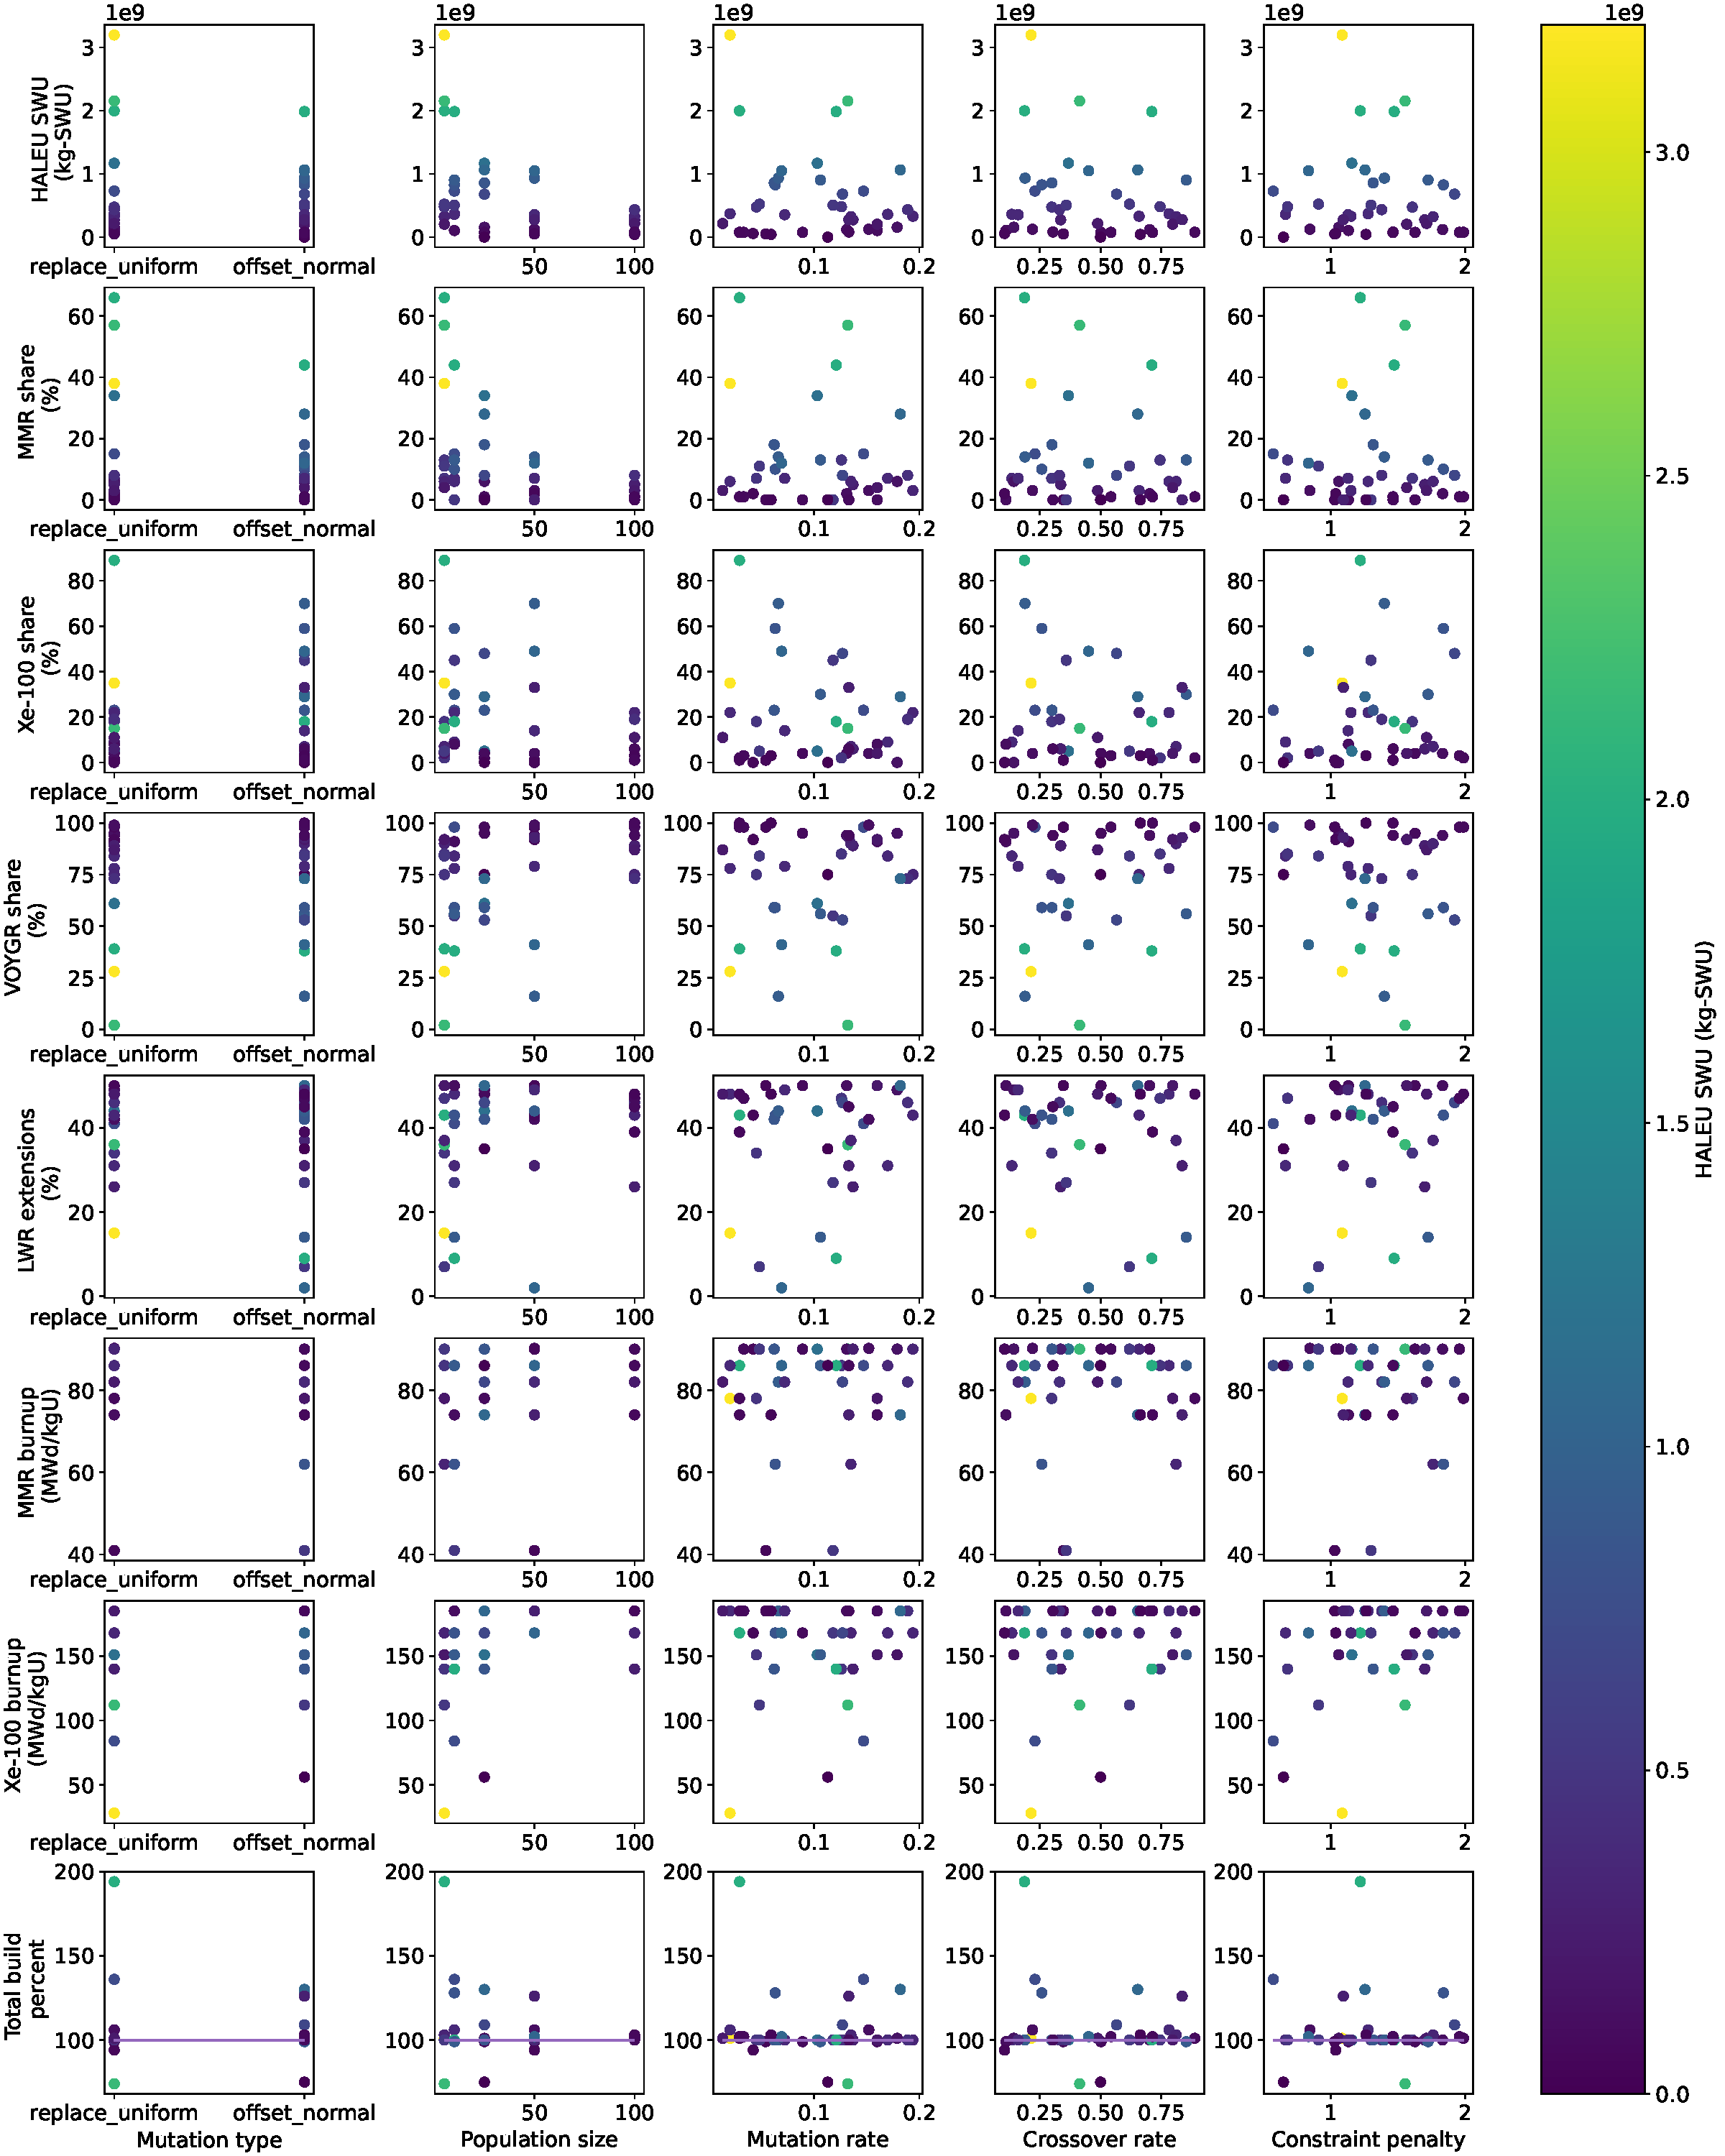
\includegraphics[scale=0.4]{soga_coarse_tuning_all_parameters.pdf}
    \caption{Results of coarse tuning for the single-objective 
    optimization.}
    \label{fig:soga_coarse_tuning}
\end{figure}

The results from the fine tuning, shown in Figure \ref{fig:soga_fine_tuning},
are not completely aligned with the results from the coarse tuning. 
The coarse tuning showed that a population size of 100 consistently performed 
better than the other population sizes, but the fine tuning showed that a 
population size of 50 performed better. Both sets of tuning runs suggested 
a population size to use, albeit suggesting different population sizes, 
but did not show any strong correlation between 
the other hyperparameters and the \gls{HALEU} \gls{SWU}. Therefore, 
we compared 
the hyperparameters and model parameters values in the five best performing 
tuning cases, based on the \gls{HALEU} \gls{SWU} required, shown in 
Table \ref{tab:soga_tuning_results}.

\begin{figure}
    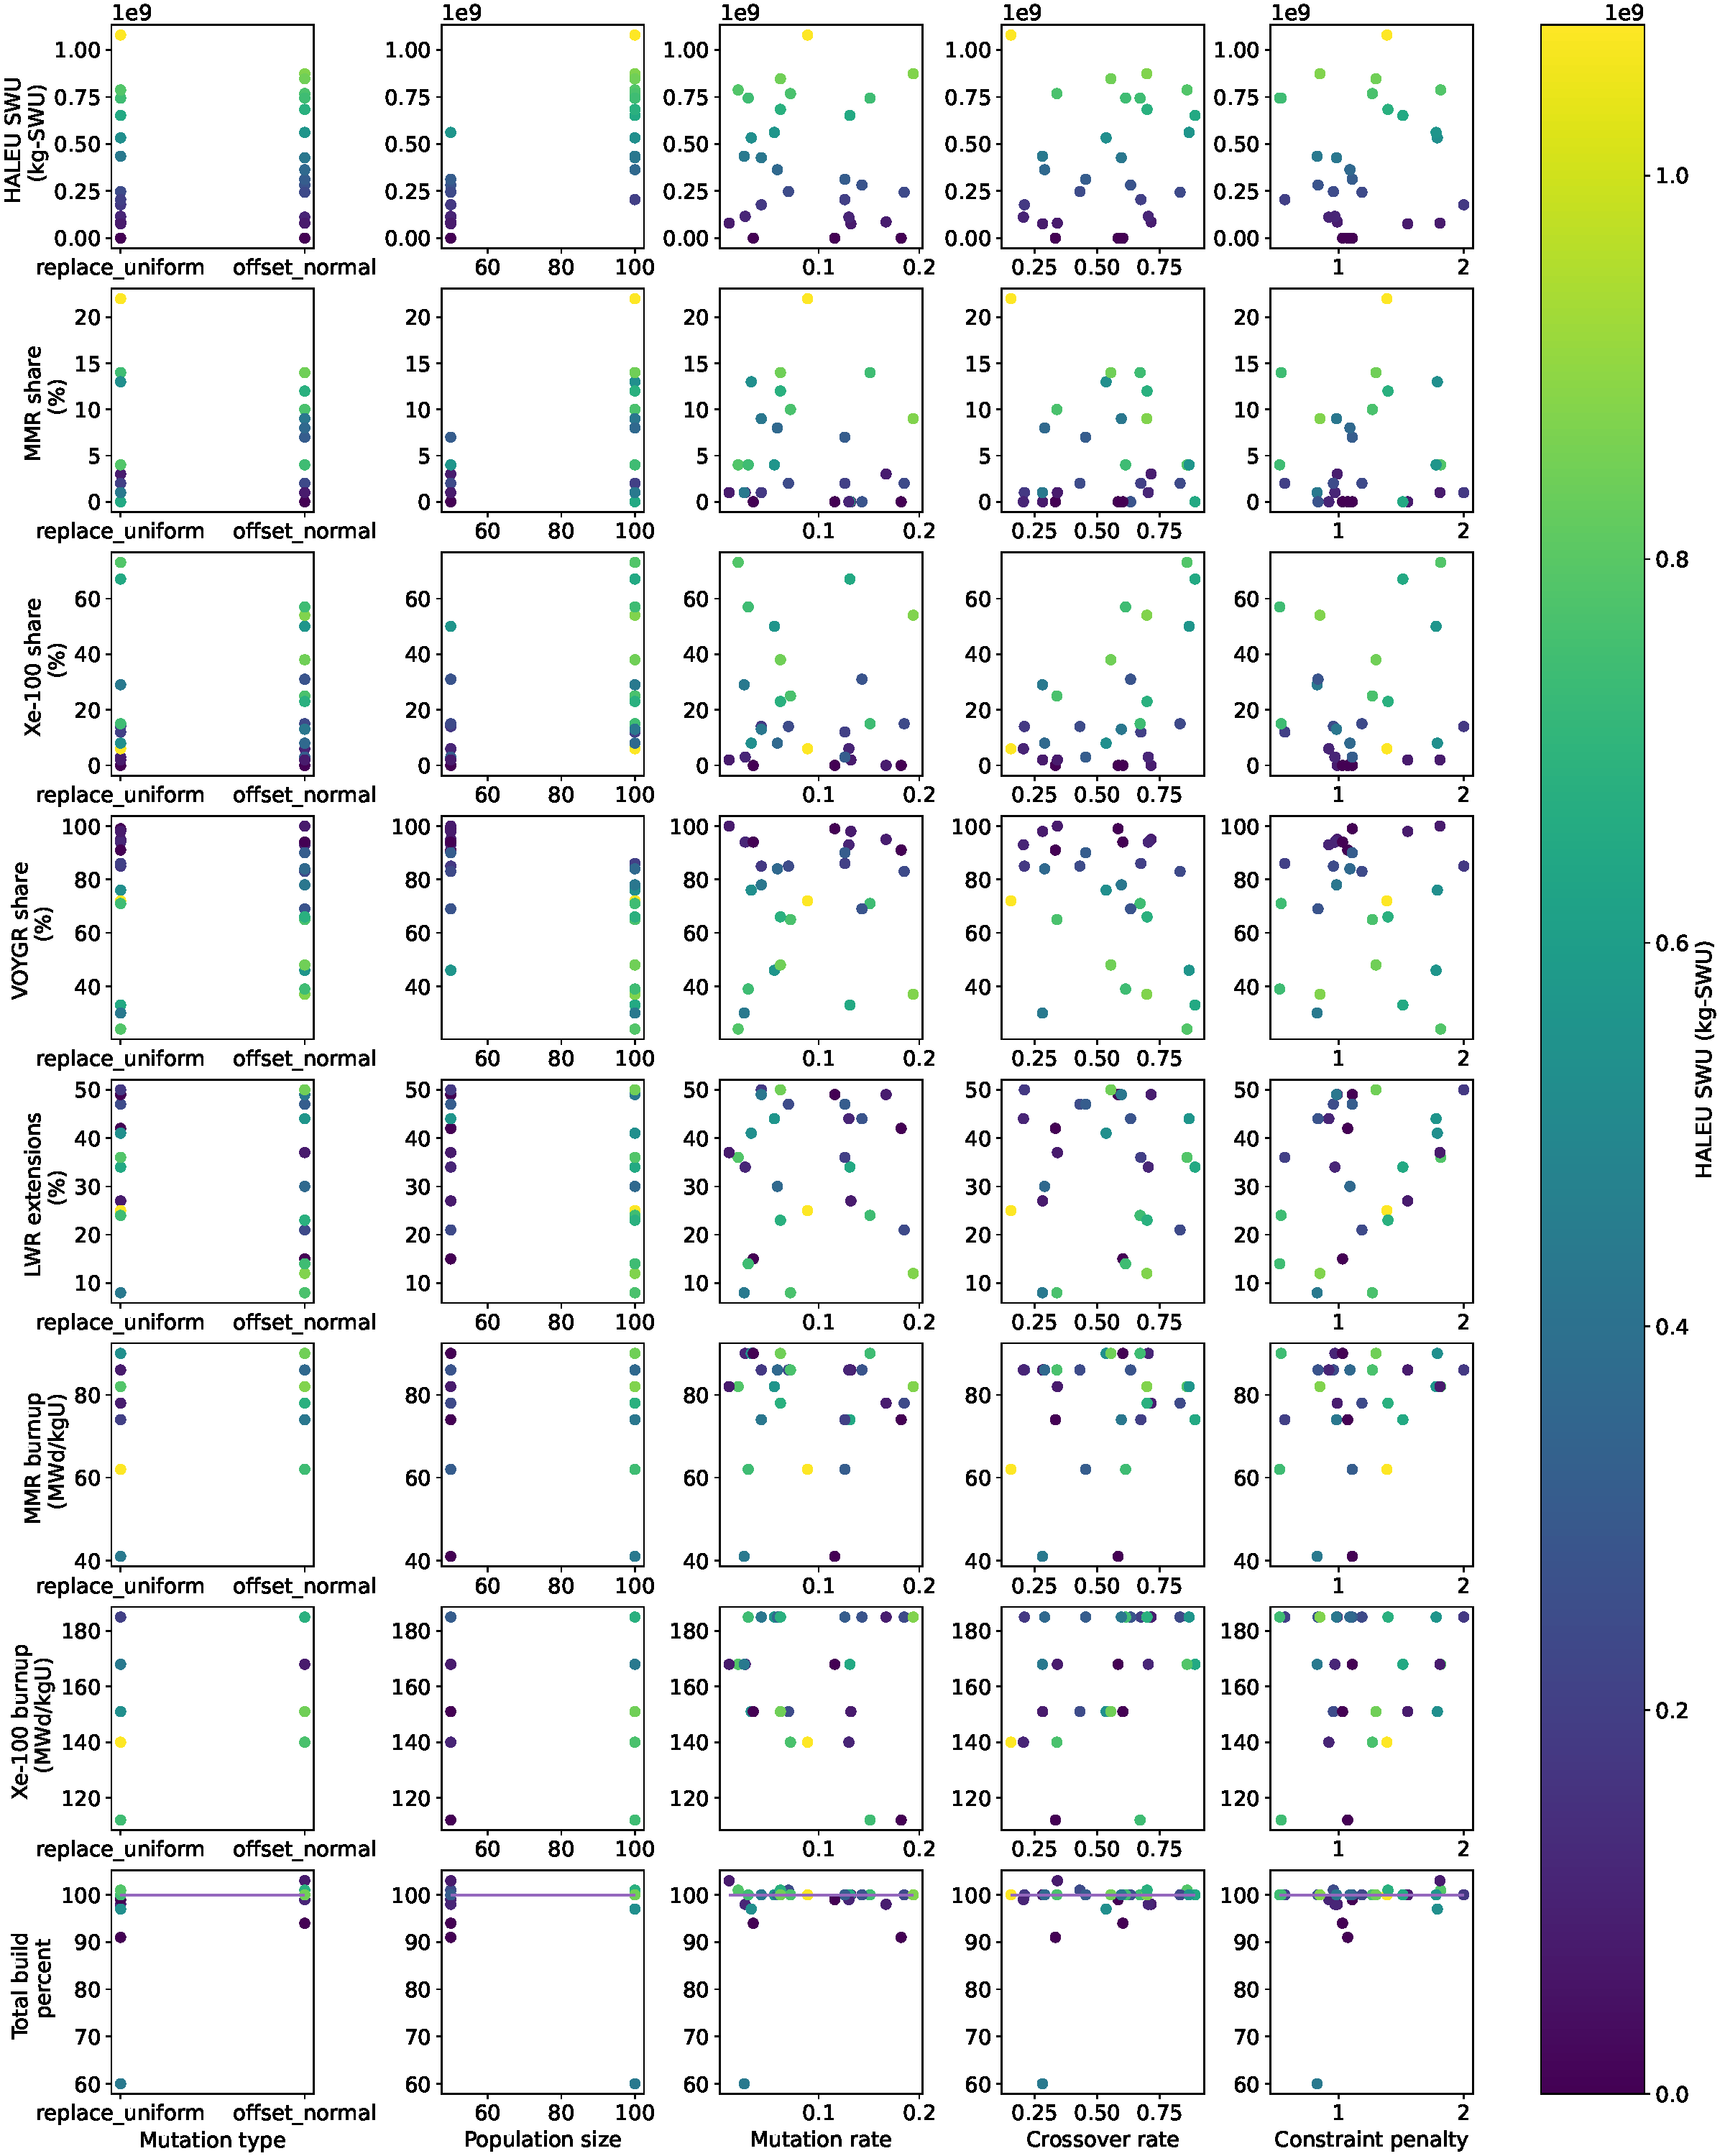
\includegraphics[scale=0.4]{soga_fine_tuning_all_parameters.pdf}
    \caption{Results of fine tuning for the single-objective 
    optimization.}
    \label{fig:soga_fine_tuning}
\end{figure}

Four of the five best performing tuning cases are able to find the 
theoretical minimum for this problem, 0 kg-SWU. However, none of the 
cases perfectly match the build share target of 100\%. Case 38 is the only 
one that at least meets the target, but it exceeds it by specifying a total 
build share of 103\%. However, this is the only tuning case that does 
not reach the theoretical minimum. 

\begin{table}
    \centering 
    \caption{Hyperparameter and model parameter values from the five best 
    performing tuning cases for the single-objective problems.}
    \label{tab:soga_tuning_results}
    \begin{tabular}{c c c c c c}
        \hline 
        & \multicolumn{5}{c}{Tuning case number} \\
        \textbf{Hyperparmeter} & 28 & 38 & 43 & 45 & 59 \\
        \hline 
        Mutation type & offset normal & offset normal & replace uniform &
        replace uniform & offset normal\\
        Population size & 25 & 100 & 50 & 50 & 50 \\
        Mutation rate & 0.113 & 0.059 & 0.182 & 0.116 & 0.035\\
        Crossover rate & 0.5 & 0.664 & 0.333 & 0.584 & 0.603\\
        Constraint penalty & 0.648 & 1.261 & 1.072 & 1.109 & 1.031\\
        \hline
        \textbf{Model Parameter} \\
        \gls{HALEU} \gls{SWU} (kg-SWU)& 0 & 4.37 $\times 10^7$ & 0 & 0 & 0\\
        VOYGR build share (\%) & 75 & 100 & 91 & 99 & 94\\
        \gls{MMR} build share (\%)& 0 & 0 & 0 & 0 & 0\\
        Xe-100 build share (\%) & 0 & 3 & 0 & 0 & 0\\
        LWR Lifetime (\%)& 35 & 48 & 42 & 49 & 15\\
        \gls{MMR} burnup (MWd/kgU) & 86 & 74 & 74 & 41 & 90\\
        Xe-100 burnup (MWd/kgU) & 56 & 185 & 112 & 168 & 151\\
        \hline 
        
        
    \end{tabular}
\end{table}

\subsubsection{Hyperparameter selection}
Based on the information in Table \ref{tab:soga_tuning_results}, we 
selected hyperparameters to use for all single-objective problems in this 
work. We selected the hyperparameters from tuning case 45, given in 
Table \ref{tab:soga_parameters}, because this tuning case reached the 
theoretical minimum for th problem and was the closest to meeting 
the total build share constraint. 

\begin{table}
    \centering
    \caption{Hyperparameters selected for single-objective optimization.}
    \label{tab:soga_parameters}
    \begin{tabular}{c c}
        \hline
        Parameter & Value \\
        \hline
        Population & 100 \\
        Constraint penalty & 1.109\\
        Crossover rate & 0.584\\
        Mutation type & replace uniform\\
        Mutation rate & 0.116\\
        \hline
    \end{tabular}
\end{table}

The tuning cases each ran a maximum of 500 evaluations to limit the 
amount of time required for each run. However, for each single-objective 
problem we run each problem for a maximum of 1000 evaluations. By 
increasing the maximum number of evaluations, we hope to ensure that 
the genetic algorithm is able to effectively find the minimum objective 
function for the problem while also meeting the total build share 
constraint by allowing more exploration of the variable space. 

\subsection{Multi-objective hyperparamter tuning}
Hyperparameter tuning for a multi-objective problem is more complicated 
than tuning for a single-objective problem. In multi-objective 
problems, there is no single best solution but rather many solutions 
that form a Pareto front \cite{adams_dakota_2021}. The points on a 
Pareto front indicate that further improvement of one objective 
results in a worsening of another objective. Therefore, to tune the 
hyperparameters of a multi-objective problem, one tunes base on the 
hypervolume of the Pareto front \cite{deb_multi-objective_2001}, because 
a larger hypervolume indicates a better exploration of the space and 
determination of equally optimized solutions. The 
hypervolume of a Pareto front is calculated by calculating the area 
between the Pareto front and a reference point. The reference point 
must be selected such that all values on the Pareto front are contained in 
the hypervolume. For multi-objective problems, we used the ``moga'' method 
in Dakota, which 
stands for Multi-objective Genetic Algorithm. Using this method, Dakota
outputs the Pareto front for the problem, which can be used to calculate 
a hypervolume with a reference point, and 
tune the hyperparameters for this problem. 

We tuned the hyperparameters based on minimizing the \gls{SWU} capacity 
to produce \gls{HALEU} and the mass of \gls{SNF} in Scenario 7.
We applied the same variable definitions 
from the single objective hyperparameter 
tuning: bounds, linear constraints, and integers for 
all variables. We observed that by using a linear equality constraint for 
the different advanced reactor build shares 
Dakota only found a single solution, as opposed to a Pareto front, because 
not all of the samples adhere to linear constraints. By using a linear 
inequality constraint, defining that the advanced reactor build share is 
at least 100\%, Dakota was able to provide multiple values for a Pareto front. 
Therefore, we used this linear inequality constraint for the tuning cases and 
the final problem run to ensure that a Pareto front can be found. Therefore, 
in addition to considering the hypervolumes resulting from each hyperparameter 
value, we will also consider how close to 100\% the total build share is 
to minimize oversupply of power.

Hyperparameters selected for tuning in this work are the 
population size, the mutation rate, and the crossover rate. Each 
hyperparameter took specific values, instead of doing a random 
search of values, because of resource limitations. The population 
sizes considered include 25, 50, and 100, mutation rates considered 
include 0.08, 0.1, 0.0116, 0.15, and the crossover rates 
considered include 0.3, 0.584, 0.8. These values 
were selected based off of the hyper parameters used for the single-objective 
problem, the default value in Dakota, or intuition. The default values for 
the population size, mutation rate, and crossover rate are 50, 
0.08, and 0.8, respectively, in Dakota. If the value of a 
hyperparameter is not specified, the Dakota default value is used.  
We ran each set of hyper 
parameters 20 times, and compared the statistics of the hypervolumes of 
the resulting Pareto fronts. From this data, we selected the 
hyperparameters to use for multi-objective optimization for this work. 

Figure \ref{fig:moga_crossover} shows the statistics of the hypervolumes 
resulting from each value of the crossover rate. All three of the 
crossover rates result in similar median values, and similar statistics. 
A crossover rate of 
0.3 results in the largest median, mean, and maximum for the 
hypervolumes. A crossover rate of 0.584 results in the smallest minimum 
hypervolume. A crossover rate of 0.8 results in the smallest median 
and mean of the hypervolumes. 

\begin{figure}
    \centering 
    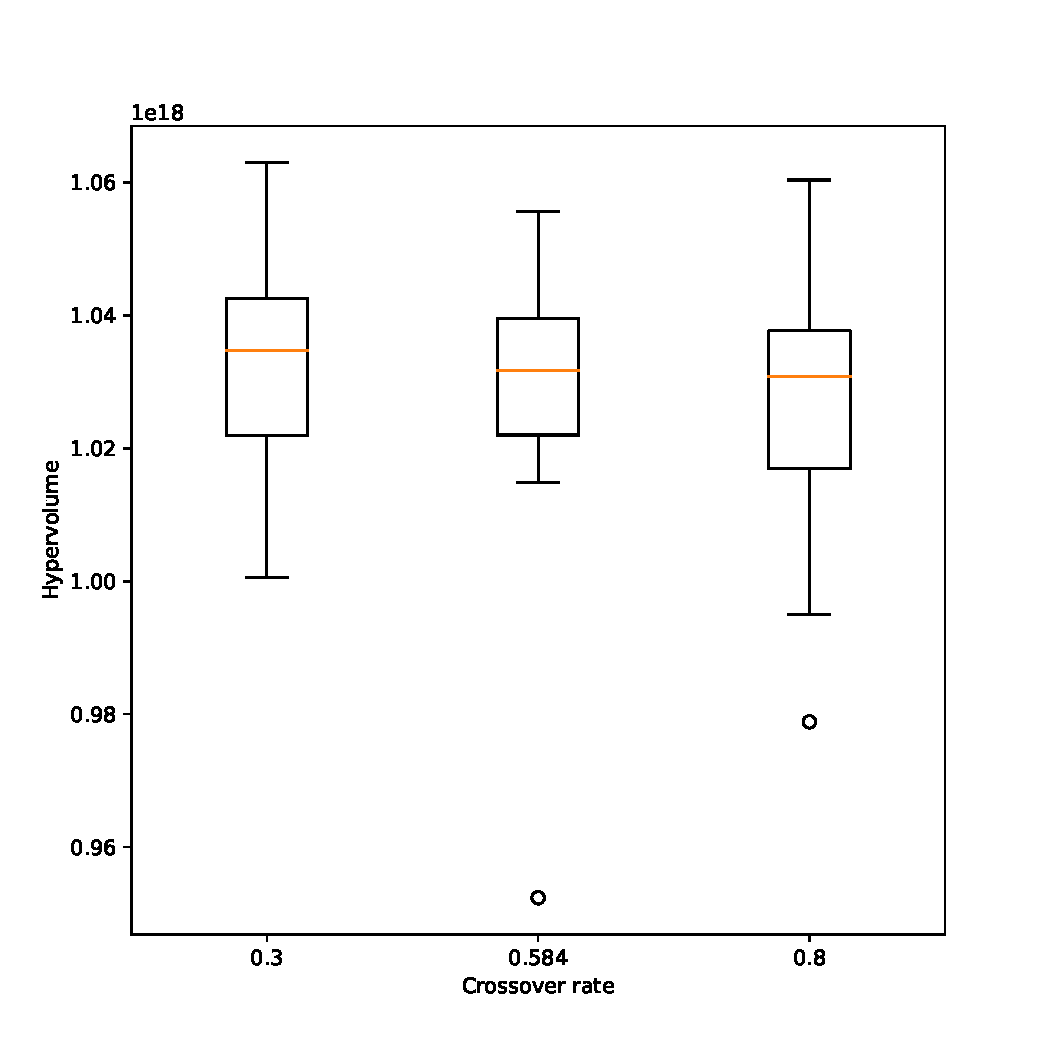
\includegraphics[scale=0.8]{moga_crossover.pdf}
    \caption{Statistics of the hypervolumes resulting from each 
    crossover rate value considered in the MOGA Tuning.}
    \label{fig:moga_crossover}
\end{figure}

Figure \ref{fig:moga_population} shows the statistics of the hypervolumes 
resulting from different population sizes. There is more observed variation 
in the statistics of this hyperparameter than the variation from varying 
the crossover rate. This observation suggests that the population size has 
a greater impact on the hypervolume than the crossover rate. A population 
size of 50 results in the largest median and first quartiles, as well 
as the smallest minimum. A population of 25 results in the largest mean 
and maximum hypervolume. 

\begin{figure}
    \centering 
    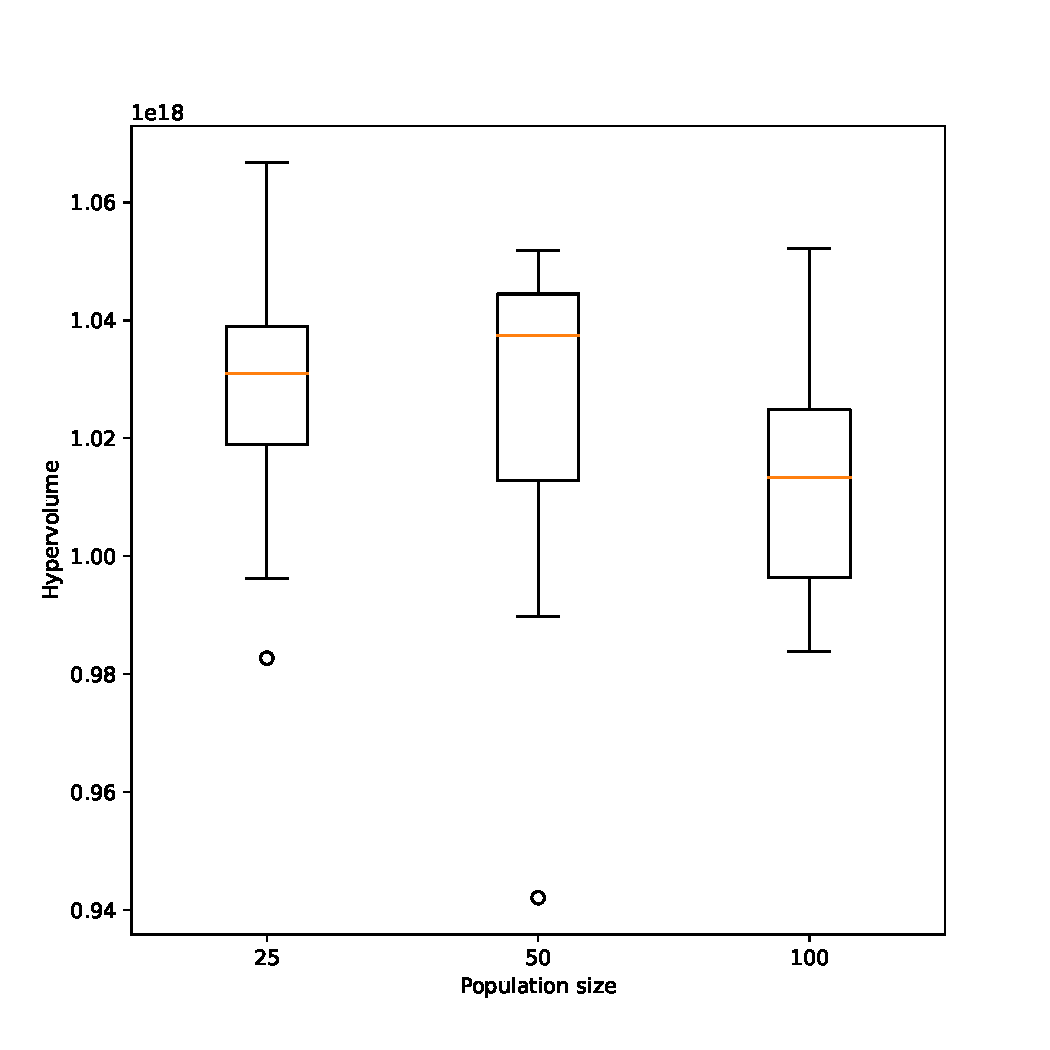
\includegraphics[scale=0.8]{moga_population.pdf}
    \caption{Statistics of hte hypervolumes resulting from 
    each population size considered in the MOGA Tuning.}
    \label{fig:moga_population}
\end{figure}

Finally, Figure \ref{fig:moga_mutation} shows the statistics of the 
hypervolumes resulting from different values of the mutation rate.
A mutation rate of 0.08 resulted in the largest mean and median of the 
values considered, closely followed by a mutation rate of 0.1, but it 
also resulted in the largest range of values. 


\begin{figure}
    \centering 
    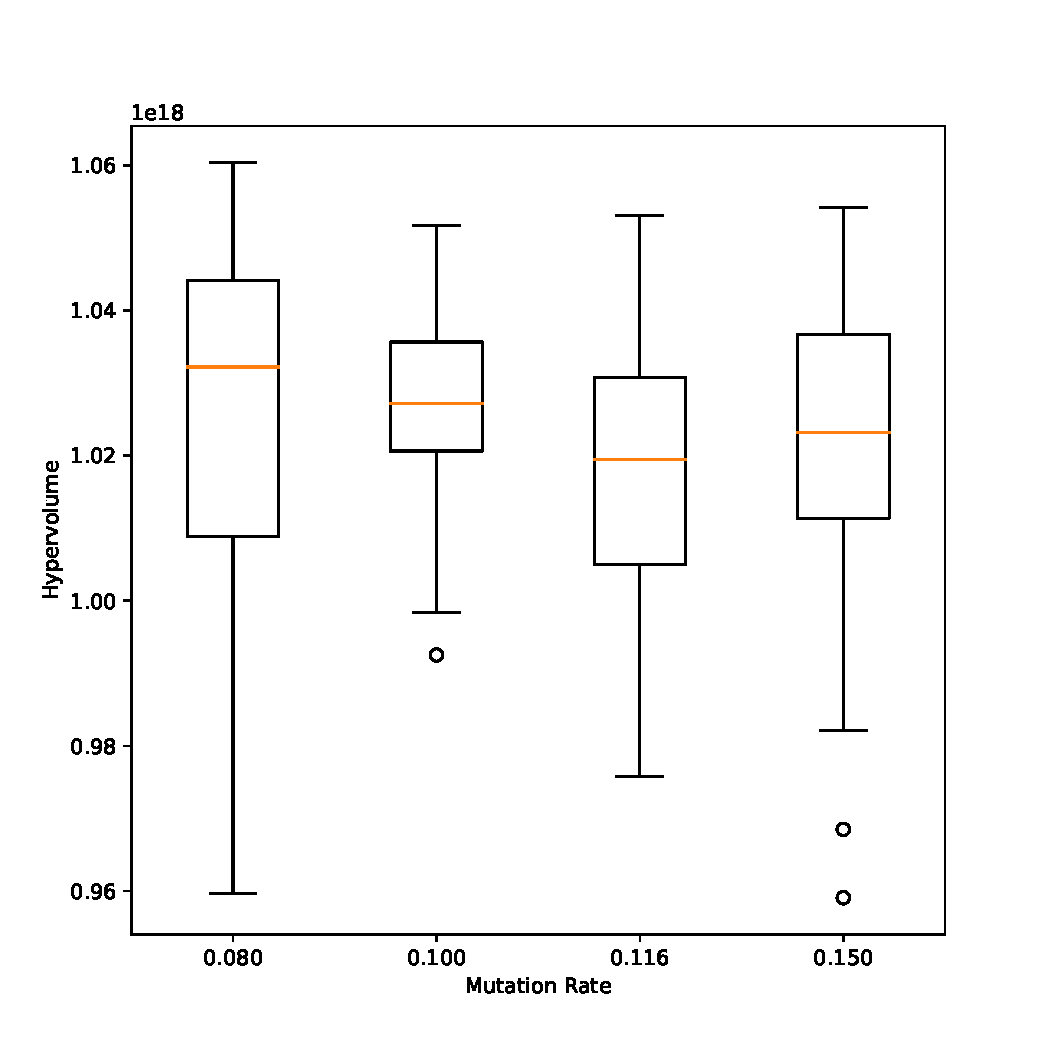
\includegraphics[scale=0.8]{moga_mutation.pdf}
    \caption{Statistics of hte hypervolumes resulting from 
    each mutation rate considered in the MOGA Tuning.}
    \label{fig:moga_mutation}
\end{figure}

\subsubsection{Hyperparameter selection}
For the multi-objective problems, we selected the hyperparameter 
values defined in Table \ref{tab:moga_parameters}. We selected 
a crossover rate of 0.3 because this parameter resulted in the 
most favorable statistics in the tuning process: the largest 
median, mean, and maximum of the resulting hypervolumes. We selected 
a population size of 25 because this population size resulted in 
the largest mean and maximum hypervolumes in the tuning cases. 
Additionally, a population size of 25 results in the highest 
values for the upper quartiles plus or minus 1.5 times the interquartile 
range (the end of the whiskers), which suggests that when this 
hyperparameter value is used again the results will continue to be 
favorable. Finally, we selected a mutation rate of 0.1 because 
although a mutation rate of 0.08 resulted in a larger mean and median 
than a rate of 0.1, it also resulted in a smaller minimum hypervolume and 
more values that are lower than those from a a rate of 0.1. Therefore, we 
selected a mutation rate of 0.1 because the hypervolumes were more 
consistent than those from a rate of 0.08. 

\begin{table}
    \centering 
    \caption{Hyperparameter values selected for multi-objective 
    optimization problems based on tuning.}
    \label{tab:moga_parameters}
    \begin{tabular}{c c}
        \hline
        Hyperparameter & Value \\
        \hline
        Crossover rate & 0.3\\
        Population size & 25\\
        Mutation rate & 0.1\\
        \hline
    \end{tabular}
\end{table}

We applied each of the hyperparameters in Table \ref{tab:moga_parameters}
to the multi-objective problem in this work. We also increased the 
maximum number of evaluations to 1500 to allow for more exploration 
of the problem space in hopes of better performance for the problems 
run. 

\section{Single-objective optimization}
\subsection{Minimize HALEU SWU}
By applying the hyperparameters to an optimization problem to minimize the 
\gls{HALEU} \gls{SWU} capacity needed by this transition scenario, Dakota
found a minimum with the values defined in Table \ref{tab:soga_ot_haleu}.
The \gls{SWU} capacity required to produce \gls{HALEU} for these input 
parameters is 4.812$\times 10^7$ kg-SWU.

\begin{table}
    \centering 
    \caption{Values resulting in a minimum \gls{HALEU} \gls{SWU} capacity for 
              a once-through transition scenario.}
    \label{tab:soga_ot_haleu}
    \begin{tabular}{c c}
        \hline
        Variable & Value \\
        \hline
        LWR Lifetime & 36\%\\
        Xe-100 build share & 0\%\\
        MMR build share & 2\%\\
        VOYGR build share & 100\%\\
        Xe-100 burnup & 151 MWd/kgU\\
        MMR burnup & 90 MWd/kgU\\
        \hline
    \end{tabular}
\end{table}

The \gls{HALEU} \gls{SWU} capacity output from this optimization is not the
theoretical minimum for this problem, and is larger than any of the values 
presented in Table \ref{tab:soga_tuning_results}. This solution results in 
a larger \gls{HALEU} \gls{SWU} capacity required because the parameters selected 
by Dakota results in a build share greater than 100\%, which artificially 
inflates the material resources needed for the transition. Additionally, 
Dakota selected a non-zero build share of \glspl{MMR}, which as the transition 
analysis and sensitivity analysis shows requires more \gls{SWU} capacity than 
the Xe-100 and VOYGR. 

The inability of the ``soga'' algorithm to properly meet the build share 
constraint in the tuning cases and in this problem identifies a significant 
disadvantage of using this method to optimize the transition. According to the 
Dakota documentation, the ``soga'' method provides a feasible solution, but
may violate the constraint as it searches the input space \cite{noauthor_dakota_2021}.
In practice, I observed that the algorithm freely explores the parameter space 
without regards to the constraint and the final solution provided is the 
iteration that best meets the constraint and minimizes the objective function.
Dakota developers suggest variation of the `constraint penalty' hyperparameter 
to force the algorithm to more strictly adhere to the constraint 
\cite{noauthor_optimization_2023}. 
However, Figures \ref{fig:soga_coarse_tuning} and \ref{fig:soga_fine_tuning}
do not show any strong correlation between the constraint penalty and how 
well the constraint is met (shown in the purple line in the bottom row of 
plots). This problem ended at 1000 iterations (the maximum allowed) and 
provided results that met the build share constraint to a similar 
extent as many of the tuning cases, which only ran a maximum of 500 iterations. 
Therefore, it is not clear if allowing more iterations will yield results that 
better meet the constraint. However, if Dakota were allowed to perform 
as many evaluations as needed to meet the convergence criteria, then 
it's possible that the constraint would be met. The Dakota manual defines some optimization 
methods that will more strictly adhere to linear constraints as they search
\cite{noauthor_dakota_2021}, such as derivative-free pattern searches. 
Therefore, a future exploration path would include use of these other 
methods to optimize fuel cycle transitions. 

With respect to the other model input parameters suggested by the optimization 
of the transition, they follow in the trends identified by the 
sensitivity analysis. The percent of \glspl{LWR} receiving license extensions
is above 25\%, the \gls{MMR} burnup is at the maximum value considered, 
and the Xe-100 burnup is near the maximum value considered. For this specific 
problem, these input parameters are not as impactful on the results as the 
build share of each reactor type. Therefore, it is reasonable that the 
results provided from Dakota do not place these variables at the very 
edge of the range of values considered. 

Because the results provided by this algorithm in Dakota do not strictly 
meet the linear constraint and do not reach the theoretical minimum for 
this problem, the results should not be accepted at face value. The results should 
be taken more as guidance on how to implement an optimized solution of 
this problem 
with respect to this objective function; maximizing the VOYGR build share in 
this transition will minimize the \gls{SWU} capacity required to produce \gls{HALEU}.

\subsection{Minimize waste mass}
By applying the hyperparameters to an optimization problem to minimize the 
\gls{HALEU} \gls{SWU} capacity needed by this transition scenario, Dakota
found a minimum with the model input parameters defined in Table 
\ref{tab:soga_ot_waste}. The minimum waste mass determined through the 
optimization is 1,736 MT. 

\begin{table}
    \centering 
    \caption{Values resulting in a minimum waste mass disposed of for 
              a once-through transition scenario.}
    \label{tab:soga_ot_waste}
    \begin{tabular}{c c}
        \hline
        Variable & Value \\
        \hline
        LWR Lifetime & 50\%\\
        Xe-100 build share & 100\%\\
        MMR build share & 7\%\\
        VOYGR build share & 11\%\\
        Xe-100 burnup & 185 MWd/kgU\\
        MMR burnup & 90 MWd/kgU\\
        \hline
    \end{tabular}
\end{table}

From Table \ref{tab:soga_ot_waste}, it is clear that more than 100\% build share
is defined, which artificially increases the \gls{SNF} mass generated from 
advanced reactors in this fuel cycle but is consistent with the results of 
the other single-objective problem for this fuel cycle. However, the build share 
percentages suggest 
a build out of Xe-100 reactors to reduce the \gls{SNF} mass generated, which 
is supported by the sensitivity analysis in Chapter \ref{ch:sa}. Additionally, 
the optimization algorithm points to a maximum in the percent of \glspl{LWR} 
receiving license extensions, Xe-100 discharge burnup, and \gls{MMR} burnup. 
These results are also consistent with the sensitivity analysis and 
modeler intuition of how to optimize for this metric. The results of the 
\gls{LWR} lifetime, \gls{MMR} burnup, and Xe-100 burnup demonstrate that this 
algorithm can perform well with respect to variables that do not have a 
linear constraint applied. 

This optimization problem converged in 590 iterations, and the best objective 
function found in iteration 437. Therefore, the hyperparameters resulted 
in a faster convergence for this problem than the previous one, despite the 
hyperparameters being tuned on the previous problem. This suggests that 
the hyperparameters for this algorithm can perform well for any problem, 
but will converge at different rates for each problem. 

\section{Multi-objective optimization}
For the multi-objective problem of minimizing the \gls{SWU} to produce 
\gls{HALEU} and the \gls{SNF} mass, Dakota identified a pareto front 
of 217 points, shown in Figure \ref{fig:once_through_pareto}. The points 
on this figure identify different values of each objective that are equally 
optimized; in order to improve one objective the other objective becomes 
worse. There is a linear trade-off between each of the objectives along this 
pareto front. 
The hypervolume of this pareto front is 1.061$\times 10^18$ using a 
reference point of (6$\times 10^9$, 2$\times 10^8$). This hypervolume is 
greater than any of the median or mean values in the hyperparameter tuning,
using the same reference point. This result suggests that these hyperparameters 
performed well in this problem. 


\begin{figure}[ht]
    \centering 
    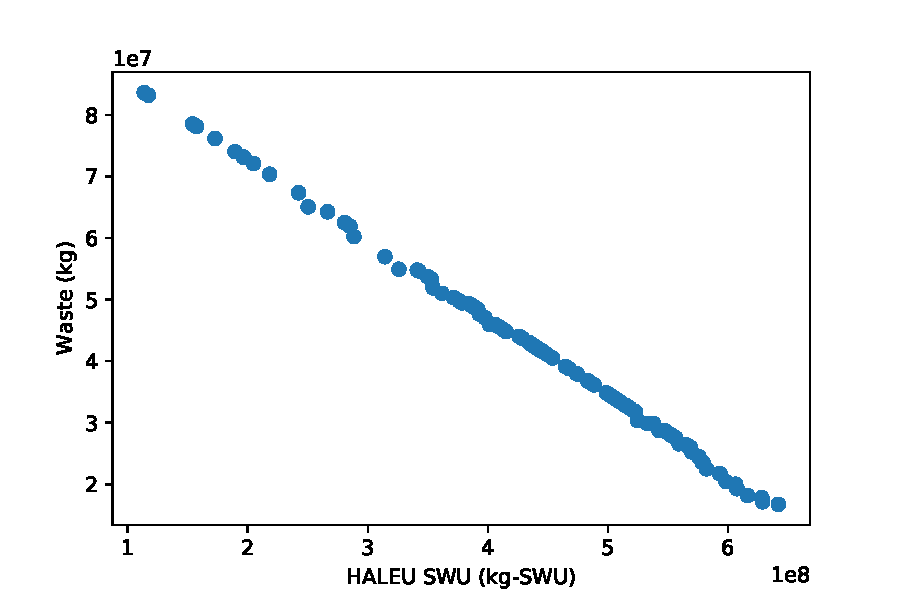
\includegraphics{once_through_pareto.pdf}
    \caption{Pareto front resulting from the multi-objective optimization 
    of the once-through transition.}
    \label{fig:once_through_pareto}
\end{figure}

The points on this pareto front have some similar model parameter values. 
Every point has a 0\% build share of \glspl{MMR} and an Xe-100 discharge 
burnup of 185 MWd/kgU. Additionally, the percent \glspl{LWR} operating 
for 80 years ranges between 47-50\%. Each of these results are very 
consistent with the results of the sensitivity analysis and the 
single-objective optimization for each problem. The \gls{MMR} discharge burnup varies 
across the range of possible values in this work because the discharge 
burnup becomes irrelevant if none of these reactors are deployed in the
transition.

The Xe-100 and VOYGR build shares vary across the pareto front. The Xe-100 
build share varies between 11-100\% and the VOYGR build share varies 
between 10-99\%. The total build share varies between 100-191\% in these 
results, with 3 of the results having a total build share of 100\%. 
These two input parameters vary the most in each of the points on 
the pareto front because they have the most effect on the results. The effect of 
these parameters explains why the pareto front is linear: each of these 
build shares has a linear relationship with the objectives (see Section 
\ref{sec:ot_oat}). Therefore, their combined effect remains linear.

Examining the Xe-100, VOYGR, and total build shares also identifies 
weaknesses in using this tool and methodology. Neither of the two reactor 
build shares reaches 0\%, which suggests that those ares of the parameter 
space were not properly explored. Additionally, 73 of the 217 (34\%) points 
on the pareto front have a total build share above 150\%. Intuition 
suggests that both objectives would be minimized with a lower total 
build share. Therefore, the total build shares further suggests that the 
genetic algorithm is not able to fully explore the parameter space. 
However, there is degeneracy in the build share of different reactors. 
Because the reactors must be built in whole numbers, multiple values of 
a build share can result in the same number of a reactor type built, 
suggesting that multiple build share percents will minimize the 
objectives. Therefore, some variation in the build share of each 
advanced reactor is a result of the degeneracy of the build 
shares. The degeneracy of the build shares is why setting a strict 
linear constraint of the build shares summing to 100\% results in 
so few points on the pareto front. However, the results of this work 
suggest that an upper limit should be applied to the linear constraint 
(instead of setting it to infinity) to produce more intuitive results. 